\documentclass[12pt]{article}
\usepackage[utf8]{inputenc}
\usepackage[margin=1in]{geometry}
\usepackage{amsmath}\usepackage{amssymb}\usepackage{multicol}\usepackage{enumitem}
\usepackage{pgfplots}\pgfplotsset{compat=1.17}
\setlength{\parindent}{0pt}
\begin{document}

\fbox{\parbox{0.97\linewidth}{\small\textbf{Final answers} (record here --- graded on the answer; show your work):\\[6pt]1.~\underline{\hspace{1.5cm}}\quad 2.~\underline{\hspace{1.5cm}}\quad 3.~\underline{\hspace{1.5cm}}\quad 4.~\underline{\hspace{1.5cm}}\quad 5.~\underline{\hspace{1.5cm}}\quad 6.~\underline{\hspace{1.5cm}}\quad 7.~\underline{\hspace{1.5cm}}\quad 8.~\underline{\hspace{1.5cm}}\quad 9.~\underline{\hspace{1.5cm}}\quad 10.~\underline{\hspace{1.5cm}}\quad 11.~\underline{\hspace{1.5cm}}\quad 12.~\underline{\hspace{1.5cm}}\quad 13.~\underline{\hspace{1.5cm}}\quad 14.~\underline{\hspace{1.5cm}}\quad 15.~\underline{\hspace{1.5cm}}}}
\vspace{0.35cm}

\begin{center}{\Large \textbf{Warm-Up: Identify $a$}}\end{center}\vspace{0.2cm}
% Warm-Up: Identify $a$
\textbf{Example (Warm-Up: Identify $a$):}

For $y=4(x-1)^2+2$, $a=4$.

\vspace{0.2cm}\hrule\vspace{0.35cm}
\textbf{Directions: State the value of $a$ for each equation and whether the parabola opens up or down.}

\begin{multicols}{2}
\begin{enumerate}[label=\textbf{\arabic*.}, start=1, itemsep=1.3cm]
  \item $\displaystyle y=3(x-1)^2+2$
  \item $\displaystyle y=-2(x+5)^2+1$
  \item $\displaystyle y=\frac{1}{4}(x-2)^2-3$
  \item $\displaystyle y=-x^2+6$
\end{enumerate}
\end{multicols}
\vspace{0.25cm}\hrule\vspace{0.35cm}

\begin{center}{\Large \textbf{Identify the Vertex}}\end{center}\vspace{0.2cm}
% Identify the Vertex
\textbf{Example (Identify the Vertex):}

For $y=-2(x+4)^2+7$, rewrite $(x+4)$ as $(x-(-4))$, so the vertex is $(-4,7)$.

\vspace{0.2cm}\hrule\vspace{0.35cm}
\textbf{Directions: Identify the vertex $(h,k)$ for each equation. Show the rewritten form when needed.}

\begin{multicols}{2}
\begin{enumerate}[label=\textbf{\arabic*.}, start=5, itemsep=2cm]
  \item $\displaystyle y=(x-5)^2+3$
  \item $\displaystyle y=2(x+2)^2-6$
  \item $\displaystyle y=-\frac{1}{2}(x-0)^2+8$
  \item $\displaystyle y=5(x+7)^2$
  \item $\displaystyle y=-4(x-9)^2-1$
\end{enumerate}
\end{multicols}
\vspace{0.25cm}\hrule\vspace{0.35cm}

\begin{center}{\Large \textbf{Full Identification}}\end{center}\vspace{0.2cm}
% Full Identification
\textbf{Example (Full Identification):}

For $y=-3(x-2)^2+5$: $a=-3$ (opens down, narrower), vertex $(2,5)$.

\begin{center}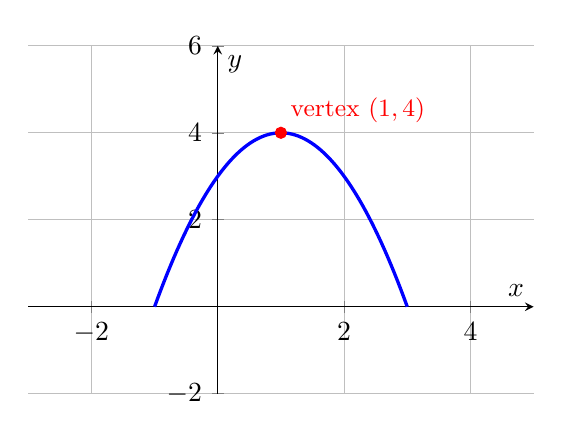
\begin{tikzpicture}
\begin{axis}[axis lines=middle,xlabel=$x$,ylabel=$y$,xmin=-3,xmax=5,ymin=-2,ymax=6,width=8cm,height=6cm,grid=both,samples=80]
\addplot[very thick,blue,domain=-1:3]{-1*(x-1)^2+4};
\addplot[only marks,mark=*,red] coordinates {(1,4)};
\node[above right,red,font=\small] at (axis cs:1,4) {vertex $(1,4)$};
\end{axis}\end{tikzpicture}\end{center}
{\small\centering The graph of $y=-(x-1)^2+4$.\par}
\vspace{0.2cm}\hrule\vspace{0.35cm}
\textbf{Directions: For each equation, state $a$, the vertex, and the direction of opening.}

\begin{multicols}{2}
\begin{enumerate}[label=\textbf{\arabic*.}, start=10, itemsep=3cm]
  \item $y=-(x-1)^2+4$ (use the graph above to confirm your answer)
  \item $\displaystyle y=2(x+3)^2-5$
  \item $\displaystyle y=-\frac{1}{3}(x-6)^2+1$
  \item $\displaystyle y=6(x+1)^2+2$
\end{enumerate}
\end{multicols}

\vspace{0.2cm}\hrule\vspace{0.3cm}
\textbf{Challenge} (same sheet):\\[4pt]
\begin{multicols}{2}
\begin{enumerate}[label=\textbf{\arabic*.}, start=14, itemsep=2.2cm]
  \item Write a vertex-form equation whose parabola opens down with vertex $(-3,5)$ and is narrower than $y=x^2$.
  \item Two parabolas both have vertex $(2,-1)$, but one has $a=4$ and the other has $a=\frac{1}{4}$. Explain how their graphs would differ.
\end{enumerate}
\end{multicols}

\newpage

\begin{center}{\Large \textbf{Answer Key --- fully worked}}\end{center}
\vspace{0.25cm}
\textbf{Procedure:} Compare the equation to the pattern $y=a(x-h)^2+k$.; Read off $a$ -- the number multiplied on the squared term.; Rewrite $(x\pm h)$ as $(x-h)$ if needed to correctly identify the sign of $h$.; Read off $k$ -- the constant added or subtracted at the end.; Write the vertex as the ordered pair $(h,k)$.; State the direction of opening: up if $a>0$, down if $a<0$..\\[8pt]
\begin{enumerate}[label=\textbf{\arabic*.},itemsep=7pt]
  \item $a=3$, opens up.
  \item $a=-2$, opens down.
  \item $a=\frac{1}{4}$, opens up.
  \item $a=-1$, opens down.
  \item Vertex $(5,3)$.
  \item Vertex $(-2,-6)$.
  \item Vertex $(0,8)$.
  \item Vertex $(-7,0)$.
  \item Vertex $(9,-1)$.
  \item $a=-1$, vertex $(1,4)$, opens down -- matches the graph shown.
  \item $a=2$, vertex $(-3,-5)$, opens up.
  \item $a=-\frac{1}{3}$, vertex $(6,1)$, opens down.
  \item $a=6$, vertex $(-1,2)$, opens up.
  \item Vertex $(-3,5)$ means $h=-3$, $k=5$; opens down means $a<0$; narrower than $y=x^2$ means $|a|>1$. One valid answer: $y=-2(x+3)^2+5$ (any coefficient with $a<-1$ works, e.g. $y=-3(x+3)^2+5$).
  \item Both share vertex $(2,-1)$ and open up, but $a=4$ makes the first parabola narrower (a vertical stretch, steeper), while $a=\frac{1}{4}$ makes the second wider (a vertical compression, flatter). At the same horizontal distance from the axis, the $a=4$ graph rises 16 times higher than the $a=\frac{1}{4}$ graph.
\end{enumerate}

\end{document}